\documentclass[12pt]{article}

%-------------------------------------------------
%   THEMES & PACKAGES
%-------------------------------------------------
\usepackage{fancyhdr}
\usepackage{lastpage}
\usepackage{xcolor}
\usepackage{pdfpages}
\usepackage{hyperref}
\usepackage{graphicx}
\usepackage{float}
\usepackage{enumitem}
\usepackage{todonotes}

%%% Custom colors & commands
\newcommand{\HRule}[1]{\rule{\linewidth}{#1}}   % Horizontal rule

%-------------------------------------------------
%   COMMON INFO
%-------------------------------------------------
\newcommand{\hmwkTitle}{R \& D Proposal}
\newcommand{\hmwkTopic}{Transfer Learning for Object Grasping}
\newcommand{\hmwkDueDate}{December 15, 2017}
\newcommand{\hmwkClass}{Research and Development}
\newcommand{\hmwkAuthorName}{Minh H. Nguyen}
\newcommand{\hmwkAuthorSchool}{Bonn-Rhein-Sieg University of Applied Sciences}
\newcommand{\hmwkAdvisorFirst}{Prof. Dr. Paul G. Pl\"{o}ger}
\newcommand{\hmwkAdvisorSecond}{Alex Mitrevski}
\newcommand{\hmwkAdvisorThird}{Maximilian Sch\"{o}bel}

\graphicspath{{../images/}}
\renewcommand{\baselinestretch}{1.2}

%-------------------------------------------------
%   MARGINS
%-------------------------------------------------
\topmargin=-0.75cm
\evensidemargin=0cm
\oddsidemargin=0cm
\textwidth=16.0cm
\textheight=22.0cm
\headsep=0.6cm

%-------------------------------------------------
%   HEADERS & FOOTERS
%-------------------------------------------------
\pagestyle{fancy}
%-------------------------------------------------
% Special first page
\fancypagestyle{firststyle} {
    \fancyhf{}
    \fancyfoot{}
    \renewcommand\headrulewidth{0.pt}
    \renewcommand\footrulewidth{0.pt}
}
%-------------------------------------------------
\lhead{\hmwkAuthorName}
\rhead{\hmwkTitle}
%-------------------------------------------------
\cfoot{Page \thepage\ of \protect\pageref{LastPage}}
%-------------------------------------------------
\renewcommand\headrulewidth{0.4pt}
\renewcommand\footrulewidth{0.4pt}

%-------------------------------------------------
%   TITLE
%-------------------------------------------------
\title{\normalsize \textsc{\hmwkAuthorSchool}   % Subtitle
    \\[2.0cm]                                   % 2cm spacing
    \HRule{0.5pt} \\                            % Upper rule
    \LARGE \textbf{\uppercase{\hmwkTopic}}
    \HRule{2pt} \\ [0.5cm]                      % Lower rule + 0.5cm spacing
    \hmwkTitle\\[0.5cm]
    \normalsize \hmwkDueDate\\
}

\author{
    \\[4.0cm]
    Author:\\
    \hmwkAuthorName\\
    \ \\
    Advisors:\\
    \hmwkAdvisorFirst\\
    \hmwkAdvisorSecond\\
    \hmwkAdvisorThird\\
}

\date{}

%-------------------------------------------------
%   BIBLIOGRAPHY
%-------------------------------------------------
\usepackage[english]{babel}
\usepackage[backend=biber]{biblatex}
\addbibresource{../RnD.bib}
%\addbibresource{proposal.bib}

%-------------------------------------------------
%   BEGIN
%-------------------------------------------------
\begin{document}
%-------------------------------------------------
    \maketitle
    \thispagestyle{firststyle}
    \newpage

%-------------------------------------------------
\section{Introduction}

    %---------------------------------------------
    \subsection{Motivation}
    \begin{itemize}
        \item Grasp planning is generally divided into analytical and empirical approaches \cite{Bohg2014}.
        \item Analytic methods often optimize some metrics which measure one or multiple properties of a robotic hand, namely dexterity, equilibrium, stability or ability to exhibit a certain dynamic behavior \cite{Bohg2014}. However, these methods often make assumptions about the object (i.e. shapes or poses) and therefore are prone to errors and does not generalize well to novel objects, while taking more time to match point clouds to known models \cite{Goldfeder2011}.
        \item Empirical or data-driven approaches generally sample from several grasp candidates and rank them according to a specific metric \cite{Bohg2014}. \todo{problem with these approaches}
        \item Mahler et al. \cite{mahler2017} proposed Grasp Quality Convolutional Neural Network (GQ-CNN) as a model to rapidly predict probability of successful grasp from depth image. Despite achieving high precision in successful grasp prediction, the model is limited in how grasps are represented: the grasp's approach vector and camera view point is presumed to be perpendicular to the table, while the gripper configuration and wrist orientation used as training input are simplified to the angle of the parallel-jaw grasp axis with respect to the table. The model is therefore insufficient in generalizing for use with mobile robots, where the camera pose often changes as the robot moves, and the grasp approach vector is not known beforehand.
        \item This research aims to extend the work by Mahler et al. \cite{mahler2017} for use with mobile robotics, specifically on the Care-O-bot 3 platform \footnote{\url{https://www.care-o-bot.de/en/care-o-bot-3.html}}, through synthesizing a new dataset using a more general grasp representation and training a new CNN model on this dataset. \todo{align motivation with project description slides}
    \end{itemize}

    %---------------------------------------------
    \subsection{Prior Work}
    \begin{figure}[h!]
        \centering
        \missingfigure{mind map}
        \caption{TODO mind map}
        \label{fig:mindmap}
    \end{figure}

	\subsubsection{Object-Grasp representation}
	Bohg et al. \cite{Bohg2014} parameterized grasps as
	\begin{itemize}
		\item the \emph{grasping point} of the object where the gripper should be aligned,
		\item an \emph{approach vector} from which the gripper shall approach the \emph{grasping point},
		\item the \emph{wrist orientation} of the robotic hand,
		\item and an \emph{initial gripper configuration}.
	\end{itemize}
	The article also categorized object-grasp representation approaches into ones which extract local (i.e. curvature, contact area with the hand) or global features (center of mass, bounding box).
	\todo{need more info}

    \subsubsection{3D grasp synthesis}
    
    \begin{figure}[H]
    	\centering
    	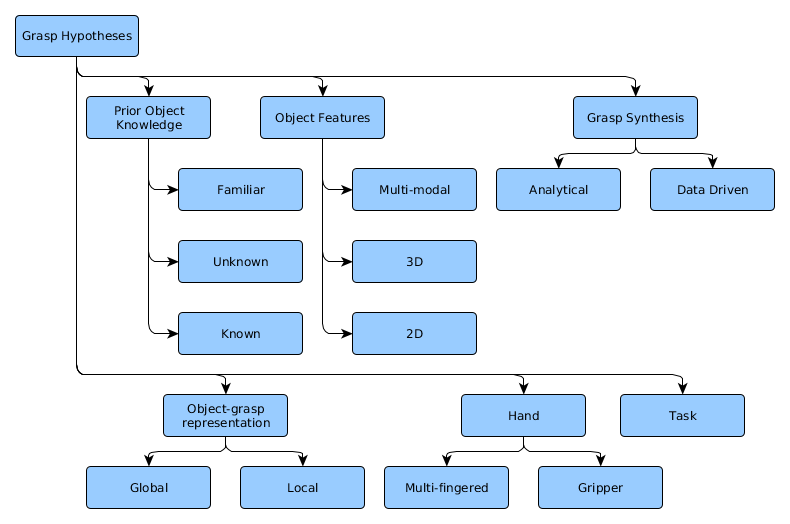
\includegraphics[width=0.8\textwidth]{bohg14-grasp_synthesis_mind_map}
    	\caption{Aspects which may influence generation of grasp hypotheses \cite{Bohg2014}.}
    	\label{fig:grasp_synthesis_mind_map}
    \end{figure}
    
    One of the key element of grasping strategies is stability. As defined in \cite{Roa2015}, a grasp is stable if position error of object caused by a disturbance disappears after the disturbance vanishes. Two important subsets of stable grasps are \emph{force closure} and \emph{form closure}. For a force closure grasp, all fingers can apply force on object to produce wrenches in all directions. A grasp that can achieve force closure with frictionless point contacts achieves form closure \cite{Sahbani2012}.

    In addition to stability, a successful grasping strategy also has to take into account task compatibility and the ability to adapt to new objects. Analytical and empirical approaches diverge in how to handle task compatibility of a grasp strategy: analytical approaches (figure \ref{fig:analytic_grasp}) find contact points and finger configuration via kinematic and dynamic formulations, while empirical approaches (figure \ref{fig:empirical_grasp}) attempt to make robots mirror human grasping \cite{Sahbani2012}.

    \begin{enumerate}
    	\item Analytical approaches are categorized in \cite{Sahbani2012} into methods which compute force-closure grasps and ones which consider task compatibility. Force-closure methods are further divided into methods which synthesize force-closure grasps and methods which attempt to find an optimal force-closure grasp using a grasp quality metric. Su\'{a}rez reviewed grasp quality metrics extensively in \cite{suarez2006}, and a more recent review was done by Roa and Su\'{a}rez in \cite{Roa2015}.
    	\item While Sahbani et al. categorized empirical approaches into techniques which focus on human observation and ones focusing on object observation \cite{Sahbani2012}, Bohg et al. argued to categorize these techniques based on the assumption of what is known about the query objects to better capture the diversity of the techniques \cite{Bohg2014}. Empirical approaches are thus divided in the latter article into ones which deal with known, familiar or unknown objects.
    \end{enumerate}

    \begin{figure}[H]
    	\centering
    	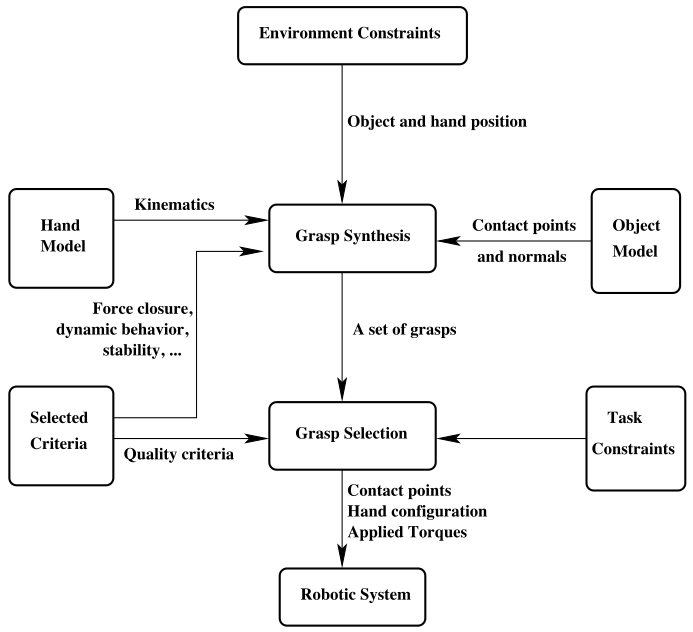
\includegraphics[width=0.7\textwidth]{sahbani12-analytic_grasp_strategy}
    	\caption{Grasp synthesis using analytical approaches \cite{Sahbani2012}.}
    	\label{fig:analytic_grasp}
    \end{figure}

	\begin{figure}[H]
		\centering
		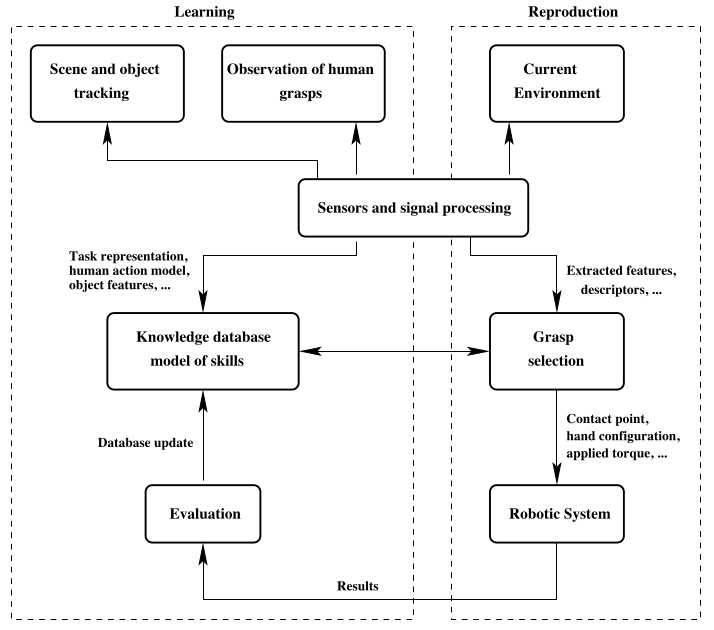
\includegraphics[width=0.7\textwidth]{sahbani12-empirical_grasp_strategy}
		\caption{Grasp synthesis using empirical approaches \cite{Sahbani2012}.}
		\label{fig:empirical_grasp}
	\end{figure}

	\subsubsection{3D grasp quality metrics}
	\todo{need more info}
    %\subsubsection{Convolutional Neural Network as feature extractor for point clouds}

    \subsubsection{Dex-Net 2.0 Data Generation}
    \begin{itemize}
    	\item Compute stable object poses from 3D mesh models from Dex-Net 1.0 \cite{mahler2016}, object meshes are rescaled to fit within the gripper physical constraints, and store poses with probability of occurrence above a threshold \todo{consider rephrase}.
    	\item Grasps are sampled using rejection sampling to ensure coverage of the object surface and is ranked and threshold using a grasp quality metric.
    	\item 2D images are generated from grasp candidates as training data with the antipodal axis aligned to the middle row of the image.
    \end{itemize}

	%---------------------------------------------
	\subsection{Hardware Specification}
	\todo{Jenny's arm and gripper specification}

	%---------------------------------------------
	\subsection{Use Case}
	\todo{Robocup@Home task description}

    %---------------------------------------------
    \subsection{Approach}
	\begin{itemize}
		\item define grasp plan representation in 3D.
		\item choose a (or several) grasp synthesis strategy to generate grasp candidates
		\item generate synthesis point cloud data with grasp based on defined representation following the Dex-Net 2.0 data generation process \cite{mahler2017}
	\end{itemize}

    %---------------------------------------------
    \subsection{Expected Results}


%-------------------------------------------------
\section{Project Plan}

    %---------------------------------------------
    \subsection{Work Packages}

    %---------------------------------------------
    \subsection{Work Schedule}
    \missingfigure{TODO Grannt chart}

\printbibliography

%-------------------------------------------------
%   END
%-------------------------------------------------
\end{document}
